Biomechanics researchers rely on numerical simulations of motion to gain understanding on a variety of scientific topics such as the physiological causes of movement disorders and their consequences on health [\addref], the estimation of non-measurable physiological quantities [\addref] and the optimality of human movement [\addref].
The musculoskeletal models used in these simulations generally have a large number of degrees of freedom and they are governed by several ordinary differential equations (ODEs) which mainly describe multibody and muscle activation dynamics.
The complexity of these systems has led scientists to formulate their simulations as optimal control problems (OCP), relying on efficient non-linear optimization software to find trajectories that fulfil a desired task while enforcing the system dynamics and minimizing a cost (e.g. motion duration, energy expenditure, matching experimental data, etc.).
Up to very recently, there was no off-the-shelf software available to the community to quickly formulate and solve such musculoskeletal OCPs, leading researchers to develop their---often simplified---own solutions.


As a result, many approaches coexist to formulate and solve OCPs in the biomechanics literature. 
The formulation, also called \comment{transcription}{discretization?}, consists in turning a continuous trajectory optimization problem into a generic discrete non-linear program (NLP) that is solved using a dedicated algorithm. 
The main family of so-called \textit{direct} transcription methods comes from numerical optimal control. 
They consist in straightforwardly choosing the state and/or the control as optimization variables at a given number of points along the trajectory and they rely on the integration of the system dynamics between these points. 

For instance, the direct collocation method has shown its efficiency in several studies investigating human motion [\addref\comment{, \`a prendre dans papier MOCO}{Sinon j'en ai un paquet dans mon Zotero que j'avais fait pour ma préparation de synthèse}]. 
It consists in approximating the integration of the system dynamics using polynomials that describe the state and control trajectories.
Its main advantages are that it leads to very sparse NLPs, that knowledge about the state trajectory can be used in the initialization, and that it handles unstable systems well \cite{diehl2006fast}. 
Its major disadvantage is that adaptive integration error control implies regridding the whole problem and thus changes the NLP dimensions, discarding its use for such application.
Direct multiple shooting is another direct method that was also applied with success in a lot of biomechanics [\addref] and robotics [\addref] studies.
Its advantages are mostly the same as for direct collocation in addition to combine integration error control with fixed NLP dimensions, as it relies on possibly adaptive ODE solvers to integrate the system dynamics.
Besides direct methods, simpler choices can be made, as in \cite{yeadon2000mechanics} [+ \addref\ Begon], where the optimization variables are instants at which a switch in the motor strategy occurs, using polynomials function (4th, 5th order) in-between, or in \cite{leboeuf2006energetic} [+ \addref\  Huchez, Mombaur, McPhee, Opensim]], where the optimization variables are the coefficients of fourth order polynomial approximations of the states, with linking conditions to enforce the continuity of the controls. 
These last approaches are less generic than the direct methods as they either require a knowledge about the state and control trajectories that one often does not have when investigating complex biomechanics issues or [discuter les méthodes type leboeuf]. 


\begin{figure}[t!]
\centering
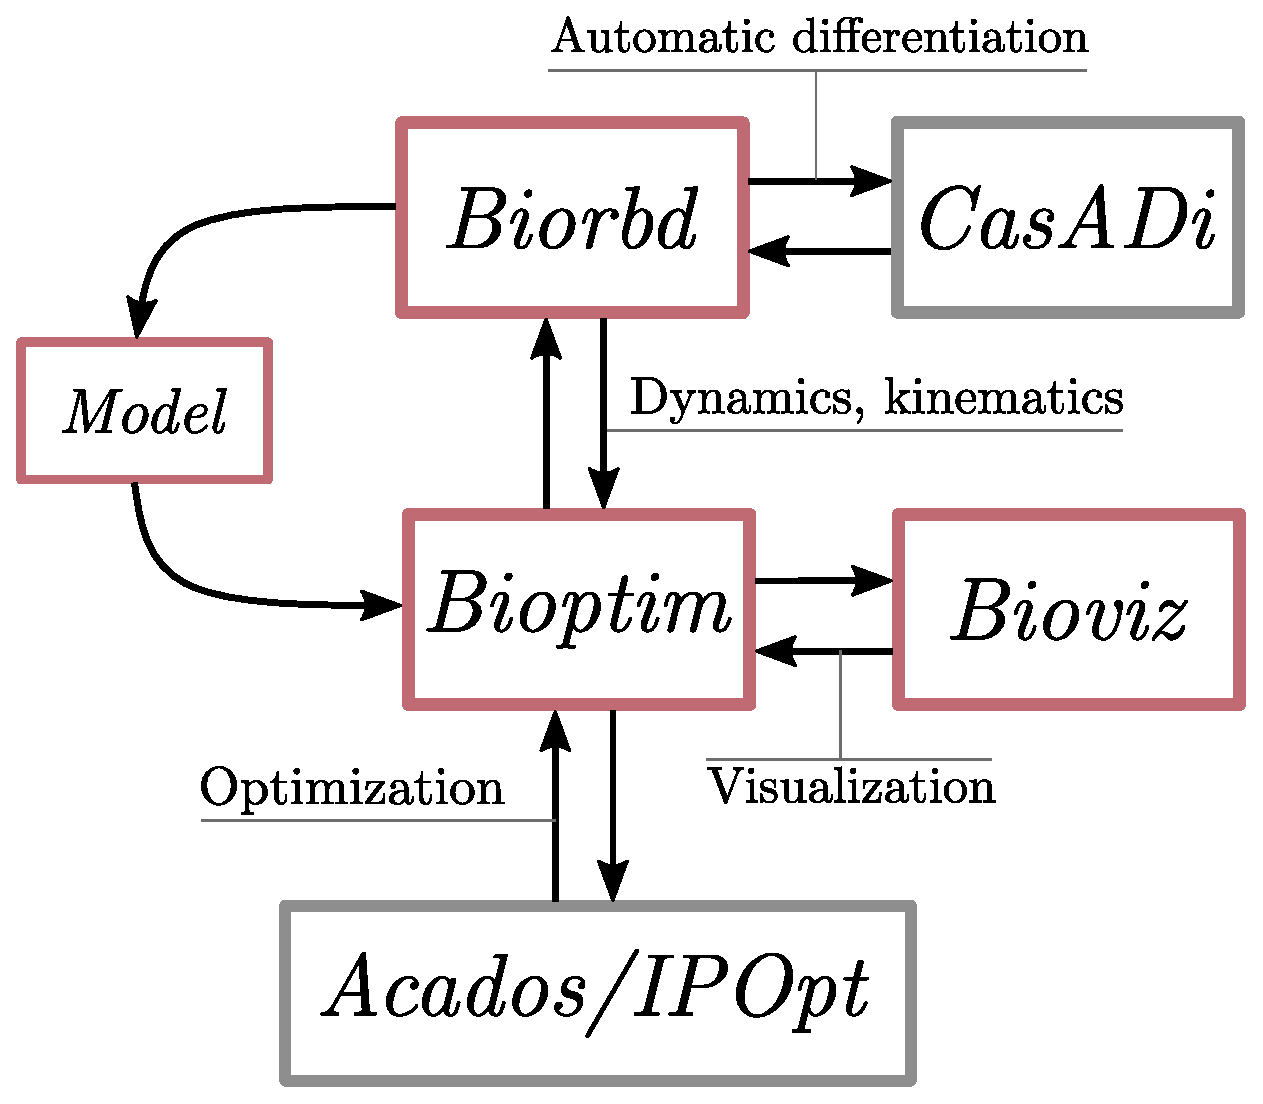
\includegraphics[width=0.9\columnwidth]{figures/dependencies.eps}
\caption{\bioptim \comment{dependencies}{Il ne semble pas que cette figure soit référencée} flowchart. \comment{The red-boxed}{Je ne suis pas sûr pour la double flèche avec bioviz. Aussi, personnellement, je les écris sans majuscules} software are developed by the S2M team. The \bioptim part is further detailed in Fig.~\ref{fig:dependencies}.}
\label{fig:dependencies}
\vspace*{-0.5cm}
\end{figure}

Concerning the non-linear solver, a variety of software exist and have been used to solve transcribed musculoskeletal NLPs.
They can use different heuristics: interior point methods (\textit{\comment{ipopt}{Il faudra s'assurer d'être consistent pour les majuscules et minuscules}}, [\addref]) or sequential quadratic programming (\textit{snopt}, \textit{acados} [\addref]), but they are all gradient based.
Therefore, derivatives of the NLP cost function and constraints are required to perform optimization.
These derivatives can be obtained by finite differences (inaccurate thus comprising convergence) or computed automatically using algorithmic differentiation [casadi].


In order to promote the use of musculoskeletal optimal control among biomechanics researcher, we identified a strong need for a dedicated tool, as shown by the recently launched \textit{MOCO} [\addref, Opensim]. 
The biomechanics community being mainly composed of software users [\addref], such a tool should request a flexible user interface written in a widely used high-level language (e.g. Python) with a low-level core (e.g. C++) for efficiency. 

To develop such a software, four interrelated components are required: \textit{i)} a musculoskeletal modeling software, with a visualization module (multibody kinematics and dynamics, muscle dynamics, etc.), \textit{ii)} a method for automatic differentiation, \textit{iii)} a discretization approach, and \textit{iv)} a nonlinear programming (NLP) solver. 
General-purpose optimal control software (e.g. GPOPS-II [\addref], Muscod-II [\addref], Acado [\addref]) address \textit{ii)} to \textit{iv)} but they need to be interfaced with a musculoskeletal modeling module and they do not provide any built-in biomechanics features (physiological cost functions, kinematic constraints, etc.). 
In that sense, the aforementioned \textit{moco}, is a welcome initiative that draws its strength from its integration with the widely used \textit{opensim}.
However, it faces the following limitations: it uses finite differences to avoid the complexity of adapting the \textit{openSim} codebase to support algorithmic differentiation, it uses direct collocation as transcription method, preventing the use of adaptive ODE solvers and it is not as flexible as required by the community, since it requires the user to develop in C++. 

%When developing such software, we should consider that human movements are often multi-staged (i.e. with different dynamics due to change in contact forces), [trouver d’autres], and models should be personalized, which may require several trials and parameter identification (e.g. isometric forces, mass properties of segments, etc.). 
%Moreover, in contrast to the inverse flow which relies on measures, solving the ordinary differential equations (ODEs) of motion may result in unanticipated behaviours, ranging from non-physiological joint angles or muscle patterns to singularities. Either convenient constraints’ definition  and XXXXX\\ 

%Lifting and relaxing OCPs\\ 
%DMS et DC\\
%Constraints vs cost\\


%While CasADi is used in MOCO mainly for its interface to ipopt (ADOL-C being used for automatic differentiation),  this tool was first and foremost designed for algorithmic differentiation and is consequently widely used for solving NLP to reduce the cost and increase the accuracy of gradient and Hessian compared to finite-difference method. Acados, a recent NLP solver dedicated to DMS, was recently launched by the same research group as CasADi taking advantage of the algorithmic differentiation for real-time applications. Some applications, such as the real-time estimation of muscle forces, presently solved by inverse approach [\addref] (from inverse dynamics to static optimization) or hybrid approach like the EMG-assisted algorithm in CEINMS [\addref], become possible [citer article François-Amedeo].


The objective of the present paper is to introduce \textit{bioptim}, an open-source optimal control software dedicated to musculoskeletal biomechanics.
\textit{Bioptim} is based on \comment{C++}{biorbd C++?} code for computational efficiency but the user interface is written in Python for flexibility and ease-of-use. 
The OCP transcription uses direct multiple shooting to preserve the possibility of using arbitrarily precise ODE solvers for the integration, which is fully parallelized for more efficiency.
\textit{Bioptim's} core is fully written in \textit{CasADi} symbolics in order to benefit from algorithmic differentiation and to exploit \textit{casadi's} interface with several non-linear solvers (\textit{ipopt, snopt}).
Also, \textit{bioptim} is interfaced with the cutting-edge solver \textit{acados}, a recent NLP solver dedicated to direct multiple shooting, intended for real-time applications.

The purpose of \textit{bioptim} is to allow fast and flexible musculoskeletal OCP formulation and solving by providing a framework with a lot of typical biomechanics problem already implemented and customizable at will.

The paper is organized as follows: first, the design and implementation of \textit{bioptim} are described.
Next, the versatility and performances of \textit{bioptim} are shown through a variety of examples available online. 
